\documentclass[a4paper]{report}
\usepackage{a4wide}
\usepackage[utf8]{inputenc}
\usepackage[T1]{fontenc}
\usepackage{parskip}
\usepackage{hyperref}
\usepackage{epsfig}
\usepackage{background}
\usepackage{mathptmx}

% To avoid tikz error, see https://tex.stackexchange.com/questions/165929/semiverbatim-with-tikz-in-beamer
\makeatletter
\global\let\tikz@ensure@dollar@catcode=\relax
\makeatother

\backgroundsetup{
scale=1,
angle=0,
opacity=1,
contents={
\includegraphics[width=\paperwidth,height=\paperheight]{images/spi-front.jpg}}
}

\hypersetup{
  colorlinks   = true,
  urlcolor     = blue,
  linkcolor    = blue,
  pdfinfo = {
    Title = {SPI Annual Report 2023},
    Author = {Software in the Public Interest, Inc.},
    Keywords = {SPI, free software, open source, FOSS, annual report, charity, non-profit, 501c3},
  }
}

\begin{document}

\title{Software in the Public Interest, Inc.\\
2023 Annual Report}
\date{July 8, 2024}

\maketitle

\newpage

\backgroundsetup{
scale=1,
angle=0,
opacity=1,
contents={
\includegraphics[width=\paperwidth,height=\paperheight]{images/spi-content.jpg}}
}

\hspace{1em}

To the membership, board and friends of Software in the Public Interest, Inc:

As mandated by Article 8 of the SPI Bylaws, I respectfully submit this annual report on the activities of Software in the Public Interest, Inc. and extend my thanks to all of those who contributed to the mission of SPI in the past year.

  \emph{-- Michael Schultheiss, SPI President}

\newpage

\tableofcontents

\newpage

\chapter{Committee Reports}
\section{Membership Committee}

\subsection{Statistics}

On January 1, 2023 we had 258 contributing and 1299 non-contributing members.  On December 31, 2023 there were 198 contributing members and 1422 non-contributing members.

\chapter{Board Report}
\section{Board Members}

Board members as of January 1, 2023:

\begin{itemize}
\item Michael Schultheiss (President)
\item Stephen Frost (Vice President)
\item Forrest Fleming (Secretary)
\item Héctor Orón Martínez (Treasurer)
\item Joe Conway
\item Milan Kupcevic
\item Jonatas L. Nogueira
\item Jeremy Stanley
\item Zach van Rijn
\end{itemize}

Board members as of December 31, 2023:

\begin{itemize}
\item Michael Schultheiss (President)
\item Stephen Frost (Vice President)
\item Zach van Rijn (Secretary)
\item Héctor Orón Martínez (Treasurer)
\item Joe Conway
\item Forrest Fleming
\item Milan Kupcevic
\item Jonatas L. Nogueira
\item Jeremy Stanley
\end{itemize}

\section{Board Changes}

Changes that occurred during the year:

\begin{itemize}

\item Joe Conway's term expired in July 2023.  Joe Conway sought, and obtained, re-election.

\item On August 14, 2023 the board voted to appoint the following officers:

\begin{itemize}
\item President: Michael Schultheiss
\item Vice President: Stephen Frost
\item Secretary: Zach van Rijn
\item Treasurer: Héctor Orón Martínez
\end{itemize}

\end{itemize}

\section{Elections}

A board membership election was conducted in July 2023.  There was 1 board seat up for election.  A nomination was received from Joe Conway.  Since there was 1 nomination for 1 board seat, no vote was required and the candidate was elected for a 3 year term.

\chapter{Treasurer's Report}

SPI will publish audited financial statements soon (approximately August 2024).

\chapter{Member Project Reports}

\section{New Associated Projects}

\subsection{Compile Farm}

\href{https://cfarm.tetaneutral.net/}{Compile Farm} is a volunteer-run project that maintains a distributed network of diverse computing resources for developers of software with OSI-approved licenses. Machines are owned and hosted by third party sponsors.

The Compile Farm Project traces its roots to a 2005 initiative by Laurent Guerby to make a wide range of computers with numerous architectures available to GCC developers. FSF France was an early sponsor.

Today, it remains a 100\% independent and volunteer-driven project, not affiliated with any sponsors or projects such as FSF, GNU, LLVM, GCC, BSD, Linux, ARM, Intel, AMD, or IBM.

\subsection{POCO: C++ Portable Components}

\href{https://pocoproject.org/}{POCO} is a collection of powerful cross-platform C++ libraries for building network- and internet-based applications that run on desktop, server, mobile, IoT, and embedded systems.

The POCO C++ Libraries have been trusted worldwide since 2005 by educators to teach the principles of programming and C++ language in education, as well as by C++ developers to build open source products and mission-critical industrial applications in a wide variety of industries.

The main goal of the project is to increase programmers' productivity by providing the missing abstractions on top of the C++ language and Standard Library, while paying attention to retain the benefits of a mature and performance-oriented programming language that C++ is.

\section{Updates from Associated Projects}

\subsection{0 A.D.}

\href{https://play0ad.com/}{0 A.D.} (pronounced ``zero ey-dee'') is a cross-platform, real-time strategy (RTS) game of ancient warfare. To win the game, one must lead an ancient civilization, gather resources, and raise a military force to defeat enemy factions. 0 A.D. is open-source software licensed under the GPL, and its art and sound assets are licensed under CC BY-SA. The game has been under continuous development by Wildfire Games, a global community of game developers, for over two decades.

In 2023, the development team worked on numerous improvements to the game engine. These include performance improvements, and upgrades of third-party libraries. Most importantly, the engine now features an experimental Vulkan graphics backend, which provides improved access to the capabilities of recent hardware. This component has received a lot of polishing work throughout the year so that we can do just that. We also tweaked the gameplay balancing to increase the variety of playing experiences.

Beyond the technical and gameplay improvements, we continued work on the organizational level as well. We began preparations for a new release of the game in 2023, but decided to put it on hold while we try to strengthen our development process. Much underground work has been performed to migrate our development environment to Git and this work continues into 2024. We hope that this modernization of our environment will make our work less energy-consuming and will facilitate the recruitment of new contributors. During the year, team members also attended some FOSS community events, most notably FOSDEM 2023.

We wish to extend our thanks to our generous donors and to SPI for helping us achieve this progress.

{\em Submitted by Aviv Sharon}

\subsection{Adélie Linux}

\href{https://www.adelielinux.org/}{Adélie} is a lightweight, musl-based, independent Linux platform for desktop and server use, committed to integrity, privacy, and user freedom.

The Adélie Linux distribution continued to deliver on its commitments. In 2023, we released our fifth beta, which brought Xfce live media, {\tt aarch64} installation media, a full set of {\tt armv7} package binaries and installation media, multi-platform Docker images, and an improved guided installer.

Over 2500 commits by 21 authors, more than double the previous year, went into this release. New tooling makes it possible to cut nightly development images and onboard new developers with ease. Generous sponsors and donors have exceeded our immediate hardware needs.

RISC-V is on the official roadmap.

Thank you to our \href{https://git.adelielinux.org/groups/adelie/-/group_members}{team}, our \href{https://www.adelielinux.org/sponsors/}{sponsors}, and our users for being part of it. Follow our \href{https://blog.adelielinux.org/}{blog} and \href{https://www.adelielinux.org/contact/}{social media accounts} to stay informed about our progress.

{\em Submitted by Zach van Rijn}

\subsection{Ankur.org.in}

In 2023 the group at \href{http://ankur.org.in/}{Ankur.org.in project} continued with the work on engaging with stakeholders in government and policy development around the digitisation of content. Additionally, the group has been focused on capacity building for computer literacy among senior citizens who have literacy and numeracy challenges.

In the past year we have participated in digital campaigns focused on building tools which help users identify synthetic content in the local language. In the near future we hope to expand this from merely text based content to audio and video content as well. This is of course subject to some grant proposals being considered by funding organisations.

{\em Submitted by Sankarshan Mukhopadhyay}

\subsection{Arch Linux}

\href{https://archlinux.org/}{Arch Linux} is a lightweight and flexible Linux distribution that tries to Keep It Simple. In 2023, the Arch Linux project achieved significant milestones across technological advancements, infrastructure improvements, and community engagement.

We have successfully migrated our packaging ecosystem to Git, with package sources now accessible on GitLab. This transition marks a major enhancement in our workflow, supported by the development of a powerful new tool called \href{https://man.archlinux.org/man/pkgctl.1}{pkgctl}. Available through devtools, pkgctl offers a user-centric design and a streamlined experience for both users and packagers, facilitating seamless interaction with all aspects of Arch Linux packaging.

Building upon the successful migration of our packaging sources to Git, we have also transitioned our bug tracking from Flyspray to GitLab. Bug reports and Merge Requests for packages or Arch Linux projects can now be managed on GitLab, enabling our contributors a modern and streamlined experience.

A lot of effort also went into various of our core projects, resulting in numerous releases. Projects such as ArchISO, arch-boxes, archinstall, mkinitcpio and many more have seen multiple updates introducing new features and enhancements.

The Arch Summit 2023 on November 4th and 5th brought together Arch Linux staff and invited guests for discussions on critical aspects of our distro.  Additionally, our participation in FOSDEM facilitated further community outreach and engagement.

{\em Submitted by Levente Polyak}

\subsection{GNU TeXmacs}

Many internal changes occurred in \href{https://www.texmacs.org/}{TeXmacs} due to evolution in the team of developers.  Most of these changes are not yet visible for the external users.

{\em Submitted by Joris van der Hoeven}

\subsection{Debian}

During 2023, \href{https://www.debian.org/}{Debian} turned 30 years old. We marked this occasion with plenty of cake and celebrations all over the world.

We also released Debian 12 (bookworm), which is a landmark release for us, since it's the first time that we've included non-free firmware on our installation media. Over recent years, installing Debian on physical hardware has become cumbersome to impossible without these firmware blobs, so while we still believe in our mission of free software, this has become necessary to allow Debian to be installed on physical hardware.

In our tradition of updating our stable releases, we've also released 3 stable point releases for Debian 11 (bullseye), as well as 3 stable point releases for Debian 12 (bookworm).

We gained 20 new Debian Developers, and 25 new Debian Maintainers who we hope will also become full project members in the future.

To stay up to date with what's happening in the Debian project, subscribe to
the \href{https://bits.debian.org/}{Bits from Debian website}.

{\em Submitted by Jonathan Carter}

\subsection{FFmpeg}

\href{https://www.ffmpeg.org/}{FFmpeg} is a complete, cross-platform solution to record, convert and stream audio and video. It is used as the foundation platform of many projects dealing with multimedia, both open source and proprietary, and is used extensively by several web-based multimedia conversion and processing services.

In the year 2023, FFmpeg released version 6.0 `Von Neumann' in February and the 6.1 point release `Heaviside' in November. A complete list of changes can be found in \href{https://git.ffmpeg.org/gitweb/ffmpeg.git/blob/HEAD:/Changelog}{the changelog}.

FFmpeg joined the GSoC 2023 program again, successfully completing two student projects. There had been developer meetings in February aligned with FOSDEM and aligned with Video Dev Days (VDD) in September.

{\em Submitted by Thilo Borgmann}

\subsection{LibreOffice}

In 2023, The Document Foundation (TDF) released two major versions of \href{https://www.libreoffice.org/}{LibreOffice}, starting with LibreOffice 7.5 in February. This release included major improvements to dark mode support, along with an improved single toolbar interface and support for data tables in Calc charts. Later in the year, LibreOffice 7.6 document themes, an accessibility check via the Sidebar, and a compact layout for Calc's pivot tables.

Throughout 2023, TDF and the LibreOffice community organised events and supported free software campaigns around the world. The LibreOffice Conference 2023 took place in Bucharest, Romania. There were also two ``Month of LibreOffice'' campaigns, which encouraged users of the software to also become contributors.

{\em Submitted by Sophie Gautier}

\subsection{MPI Forum}

The Message Passing Interface (MPI) API is one of the most widely used programming abstractions for High-Performance Computing (HPC) and is used on basically all HPC systems world-wide. Its specification is curated and advanced by the \href{https://www.mpi-forum.org/}{MPI Forum}, a group of volunteers from industry, academia, compute centers and national laboratories, which meets regularly to discuss technical and strategic directions of MPI. Further, the work is connected to the yearly EuroMPI conference, an academic conference with presentations on new directions and evaluations of the current standard. Both, the MPI Forum and the EuroMPI conference series are part of the Software in the Public Interest (SPI).

On the forum side, the MPI forum ratified the latest MPI standard, Version 4.1, on November 2, 2023, and made it available publicly. This updated version includes new features, such as automatic message buffering, memory management for accelerated systems, and improved error handling, alongside many clarifications and readability improvements. Implementations of these new features is on its way in most MPI distributions and are either already available to the user community or will be soon. In addition to many online meetings, the forum also met two times in hybrid fashion, with physical locations in Boston, USA (March 2023) and Bristol, UK (September 2023).

On the EuroMPI side, the conference was held last year from September 11-13, 2023, in Bristol. It was hosted by the University of Bristol and held in conjunction with both an MPI Forum meeting and the annual IWOMP conference, which is an academic conference that focuses on a closely related standard in HPC, called OpenMP. MPI and OpenMP have many synergies so they have been meeting back-to-back at the same venue for several years. The combined conferences featured 32 speakers and were attended by 83 researchers, and were, once again, an ideal place for discussions on future directions of MPI and its related technologies.

{\em Submitted by Martin Schulz}

\subsection{ns-3}

\href{https://www.nsnam.org}{ns-3} is a discrete-event, packet-level network simulator with an emphasis on networking research and education.

In 2023, ns-3 published three software releases of the simulator, thanks to submissions from thirty-one contributors.  Development of new modeling capabilities was focused on the Wi-Fi module, the LR-WPAN module for wireless personal area networks, and propagation models for cellular simulations.  ns-3 also mentored three student projects in the 2023 edition of Google Summer of Code.  After three years of online annual academic workshops due to the pandemic, the project held a hybrid workshop in the Washington D.C. area, featuring sixteen technical paper presentations and numerous short talks and tutorial sessions.

{\em Submitted by Tom Henderson}

\subsection{OFTC}

\href{https://oftc.net/}{OFTC}'s IRC network is continuing to happily run along.

{\em Submitted by Christoph Berg}

\subsection{Open Bioinformatics Foundation}

The \href{https://www.open-bio.org/}{Open Bioinformatics Foundation} (OBF), founded in 2001, is a non-profit, volunteer-run group that promotes open source development and open science in biological research. OBF is led by an \href{https://open-bio.org/board/ }{elected Board that currently includes 9 members}, with Peter Cock as the president. There have been no changes to the OBF Board in the past year.  During our public Board meeting on 2023-12-19, three board members were re-elected: Peter Cock (President), Heather Wiencko (Treasurer), and Hilmar Lapp (Member at Large).

In 2023, OBF awarded 6 Event Fellowships over three rounds, as part of its program to increase diverse participation at events that promote open science.

On March 14, 2023, the OBF hosted an ISCBacademy webinar in which Hannah Wei -- co-founder of the Patient-Led Research Collaborative–-- gave a talk on ``Re-Thinking the Patient's Role in a Learning Health System: Lessons from the Patient-Led Research Collaborative'' (\href{https://youtu.be/M2vAotWKd_Q}{video}). Another ISCBacademy webinar on October 3, 2023, which was jointly sponsored by the Bio-Ontologies COSI, featured Sierra Moxon speaking about ``LinkML: an open data modeling framework, grounded with ontologies'' (\href{https://youtu.be/CwyncsMMdNA}{video}).

OBF's annual Bioinformatics Open Source Conference, BOSC 2023, was part of ISMB/ECCB 2023 (in Lyon, France, and online). ISMB/ECCB 2023 attracted a near-record number of attendees, with over 2100 in person and about 900 more online. Approximately 200 people participated in BOSC sessions. In addition to 43 talks and 49 posters, BOSC 2023 featured two keynotes: Sara El-Gebali, who spoke about ``A New Odyssey: Pioneering the Future of Scientific Progress Through Open Collaboration'' and Joseph Yracheta, who spoke about ``The Dissonance between Scientific Altruism \& Capitalist Extraction: The Zero Trust and Federated Data Sovereignty Solution''. A joint session brought together BOSC and the Bio-Ontologies COSI. The conference closed with a panel on Open and Ethical Data Sharing. It was preceded by the BOSC/OBF CollaborationFest, a collaborative work event that brought together about 40 participants interested in synergistically combining ideas, shaping project plans, developing software, and more.

BOSC 2024, the 25th annual BOSC, will take place July 15-16, 2024, in Montréal, Canada (with an online option), and will be followed by a CollaborationFest.

{\em Submitted by Heather Wiencko}

\subsection{OpenEmbedded}

\href{https://www.openembedded.org/}{OpenEmbedded} is a build system that creates custom Linux distributions for devices running Linux. Traditionally used for creating images for embedded devices, OpenEmbedded is now used all over to create small images for Internet of things (IoT) devices, to large images pushing into the desktop space.

In 2023 we provided travel support to a developer who presented Software Bill of Material work at FOSDEM. We also arranged an OpenEmbedded workshop after FOSDEM.

{\em Submitted by Philip Balister}

\subsection{OpenZFS}

\href{https://openzfs.org/}{OpenZFS} is an open-source storage platform that includes the functionality of both traditional file systems and volume manager.

OpenZFS held its annual Developer Summit in October 2023. 6 presentations from people at 5 companies were viewed by 35 in-person attendees and thousands online. Planning for the October 2024 event is underway.

We also published the v2.2.0 release and 10 patch releases with bug fixes and small features (8 for v2.1.x, 2 for v2.2.x).

{\em Submitted by Karyn Ritter}

\subsection{PMIx}

The \href{https://pmix.github.io/}{PMIx organization} is a collection of academics, researchers, and vendors who develop and maintain cutting-edge technology for deploying, managing and improving interoperability between most-demanding High Performance Computing (HPC) environmental management software, notably for the deployment and runtime management of distributed applications, and their interoperability with launch managers and batch schedulers. The organization supports the development and release of the PMIx standard, and is closely associated with the Open PMIx and PRTE reference implementations.

In 2023:

\begin{itemize}

\item The organization held 4 Administrative Steering Committee meetings. The meetings include all stakeholders during two 3 hour sessions, during which the eligible members of the ASC vote on inclusion and modification of the PMIx standard document. The organization also held elections to renew its chairs and secretaries, as well as updated bylaw documents.

\item Multiple working groups have been active and proposed amendments to the standard with respect to 1) making the document implementation neutral, better separating API and concepts from the reference implementation design; 2) introducing an ABI to enhance the portability of PMIx application and system services; 3) the expansion of the standard to support malleable applications, that is, applications that can react to runtime changes to the number of available allocated resources.

\item During the reporting period, the organization published two new revisions of the PMIx Standard. PMIx v5.0, is a feature revision of the standard including the standardized ABI. PMIx v4.2 is a bugfix release that backports some of the errata changes from v5.0 to the backward compatible v4 line of standard.

\end{itemize}

{\em Submitted by Aurelien Bouteiller, PMIx ASC co-chair, on behalf of the PMIx ASC}

\subsection{PostgreSQL}

\href{https://www.postgresql.org/}{PostgreSQL} is a powerful, open-source relational database management system that emphasizes extensibility, robustness, and SQL compliance.  PostgreSQL's open-source ecosystem continues to experience significant growth, attracting new users, contributors,and innovative solutions.  This vibrant community propelled PostgreSQL to the top of the 2023 Stack Overflow developer survey, with accolades for being the most admired, desired, and popular database.

The release of PostgreSQL 16 in September 2023 delivered a wealth of enhancements. Highlights include support for logical replication from physical standby servers, advancements in query parallelization for improved performance, and expanded SQL/JSON syntax for greater flexibility. Additionally, PostgreSQL 16 prioritizes observability with the introduction of "last usage" timestamps for indexes and tables, alongside a new system view for gathering detailed I/O statistics.

Fueled by expanded attendance at PostgreSQL events, we're witnessing a renewed passion for PostgreSQL extensibility. Contributions are flourishing in various areas, particularly AI-related technologies, promising even greater innovation in 2024. This enthusiasm is further bolstered by a growing pool of project contributors and committers, solidifying confidence in the long-term health and vibrancy of the PostgreSQL project.

{\em Submitted by Robert Treat}

\subsection{Privoxy}

In 2023, \href{https://www.privoxy.org/}{Privoxy} 3.0.34 was released which fixed a couple of bugs and came with a new client-body-tagger action which creates tags based on the content of the request body.

For the first time project money was used to fund development: WolfSSL support was added and tests based on the curl test suite were written.

{\em Submitted by Fabian Keil}

\subsection{Swathanthra Malayalam Computing (SMC)}

\href{https://smc.org.in/}{Swathanthra Malayalam Computing} (SMC) works as an umbrella organization of various free and open-source language technology projects in Indian languages.

SMC volunteers actively participated and collaborated in various community events throughout the year, including India FOSS 3.0 (Bangalore), DebConf 2023 (Kochi), FreedomFest 2023 (Trivandrum), Wikimania 2023 (Singapore), State of the Map Asia 2023 \& FOSS4G Thailand (combined event), and Wiki Conference Kerala (Thrissur).

Font Development and Maintenance:

\begin{itemize}

\item Continued maintenance and support for existing SMC font packages like Manjari, Nupuram, Gayathri, and Chilanka with new version releases.

\item Development efforts progressed on a new typeface named Malini.

\item SMC fonts were re-listed on Google Fonts after resolving identified bugs and through consistent follow-up.

\item A detailed 40-page specimen for the Nupuram font was released.

\item A long-standing date sign issue in SMC fonts was addressed to resolve user concerns, particularly within LibreOffice.

\end{itemize}

We also performed significant software development and had a number of academic achievements.

{\em Submitted by Santhosh Thottingal}

\subsection{systemd}

\href{https://systemd.io/}{systemd} is a suite of basic building blocks for a Linux system. It provides a system and service manager that runs as PID 1 and starts the rest of the system. In 2023 we published three major releases of systemd and 61 point releases with bug fixes. We merged 6814 commits (up from 5428 in 2022) from a total of 368 contributors. We organized a \href{https://archive.fosdem.org/2023/schedule/track/image_based_linux_and_secure_measured_boot/}{devroom at FOSDEM in February}, we organized the \href{https://uapi-group.org/docs/minutes/2023-09-12__image-based-linux-summit/}{Image-Based Linux Summit} and we participated in \href{https://cfp.all-systems-go.io/all-systems-go-2023/schedule/}{All Systems Go!} in Berlin in October. We used our SPI funds to pay a contractor to improve our documentation, adding versioning to all options in manpages and to the documentation rendered on our website. We continue to hold a biweekly maintainers meeting and the project is maintaining a steady pace of development.

{\em Submitted by Luca Boccassi}

\subsection{The Mana World}

\href{https://www.themanaworld.org/about}{The Mana World} organisation has rebranded as Manasource, a cooperative group of development projects focused on free open source videogame software. Besides publishing other software, Manasource aims to build its own complete 2D MMORPG platform in its main game project: The Mana World.

The Mana World is nearly ready to move to an upgraded server engine that will solve a lot of issues and facilitate future development. New content continues to be added to the game as always.

Moubootaur Legends completed both the player story arch, as well as the world story arch. This is a major landmark in the game development, and it allows the team to focus on polishing the game, fixing the countless bugs which have crept in the past years, as well as completing the translations to Portuguese and Spanish, which are the current focus.

Source of Mana continues to build its foundations with many improvements to UI, combat, NPCs, navigation and an `overworld' feature in the form of a navigable and interactive world map.

Find us on our \href{https://forums.themanaworld.org/}{forums} to stay up to date with news, development and our community!

{\em Submitted by the Mana Team}

\subsection{Translatewiki.net}

\href{https://translatewiki.net/}{Translatewiki.net} is an online translation platform for free and open-source projects, supported by a community of volunteer translators.  Our platform has maintained stable activity, with around 1,600 active yearly translators contributing approximately 665k translations. We welcomed over one thousand new translators and onboarded 57 new software projects or their components.

We integrated the Wikimedia Foundation's \href{https://www.mediawiki.org/wiki/MinT}{MinT translation service} to expand translation suggestions and installed a new discussion system to replace our previous buggy and unmaintained one. Additionally, we onboarded a new deployer, improved error logging, and simplified deployments by removing an extension that frequently caused issues and required extensive maintenance.

{\em Submitted by Niklas Laxström}

\subsection{Tux4Kids}

\href{https://tuxpaint.org/}{Tux Paint} has two releases:

\begin{itemize}

\item 0.9.30 (May 2023) added support for a sizing option to some Magic tools, a small improvement to text legibility on the UI buttons, and Tux Paint Config. (settings tool for parents/teachers) is for the first time available on Haiku OS.

\item 0.9.31 (July 2023) introduced a few new Magic tools, fuzzy-edged erasers, and the ability to create `templates' (backgrounds that can be drawn over; using the eraser tool reveals the template) directly within Tux Paint (from the `Open' dialog).  Also, the UI font may now be configured.

\end{itemize}

Tux Paint continues to be active on social media.

{\em Submitted by Bill Kendrick}

\appendix
\chapter{About SPI}

SPI is a non-profit organization which was founded to help organizations develop and distribute open hardware and software. We encourage programmers to use the GNU General Public License or other licenses that allow free redistribution and use of software, and hardware developers to distribute documentation that will allow device drivers to be written for their product.

SPI was incorporated as a non-profit organization on June 16, 1997 in the state of New York. Since then, it has become an umbrella organization for projects from the community.

In 1999, the Internal Revenue Service (IRS) of the United States government determined that under section 501(a) of the Internal Revenue Code SPI qualifies for 501(c)(3) (non-profit organization) status under section 509(a)(1) and 170(b)(1)(A)(vi). This means that donations made to SPI and its supported projects are tax-deductible as charitable donations for US taxpayers.

\newpage

\pagestyle{empty}

\backgroundsetup{
scale=1,
angle=0,
opacity=1,
contents={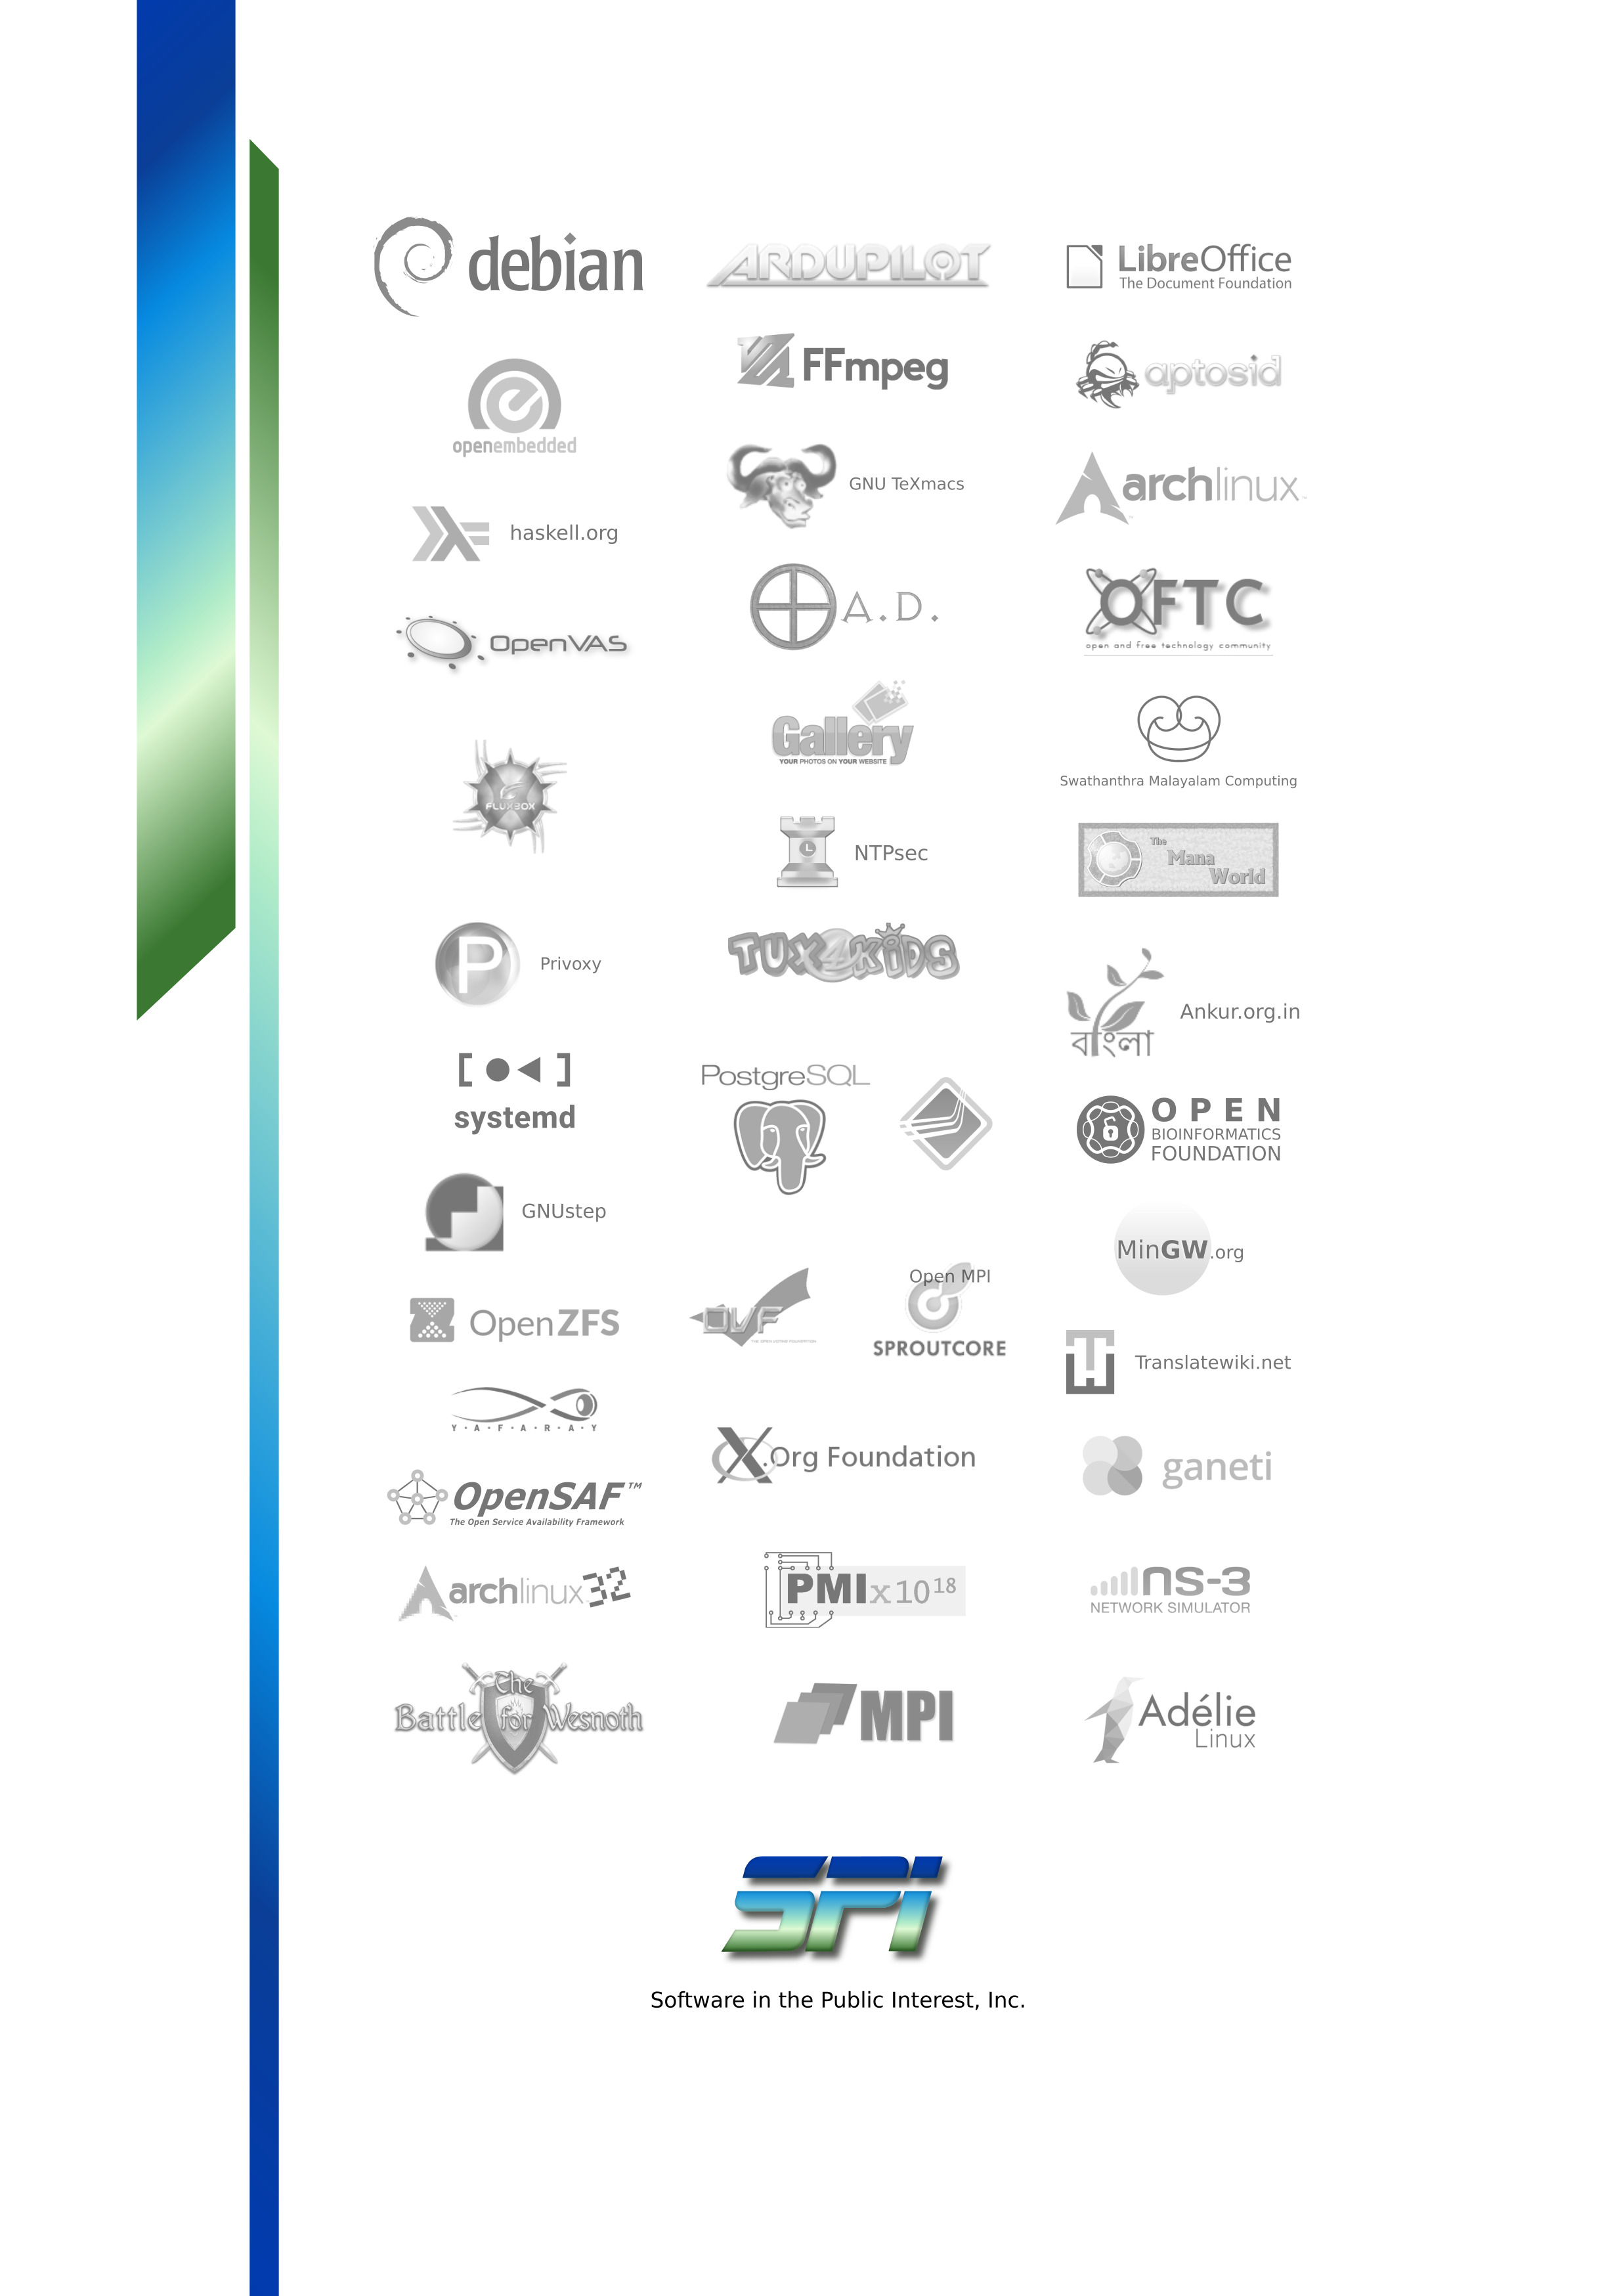
\includegraphics[width=\paperwidth,height=\paperheight]{images/spi-back-2022.jpg}}
}

\null

\end{document}
% Keep this at the bottom, thanks.
% Local Variables:
% TeX-master: "report"
% End:
